\chapter{Experiment}

The \gls{caes} at the University of Melbourne has be assembled over a number of years. The experimental cycle can be divided into several parts which will be briefly descibed in this chapter. More details of the various experimental apparatus can be found in the group's recent papers \cite{bell_slow_2010, mcculloch_arbitrarily_2011, saliba_spatial_2012} and theses \cite{mcculloch_towards_2012, sheludko_shaped_2010, saliba_partially_2011}.


\section{Magneto-Optic Trap}

The first stage of the experiment is trapping rubidium atoms in a \gls{mot}. An oven is used to create Rubidium vapour with a temperature around 350K which is collimated and directed down the axis of the Zeeman slower. The Zeeman slower slows the atoms down such that when they reach the main chamber they can be trapped by the combined magnetic and optical traps.


\subsection{Rubidium Oven}

\begin{wrapfigure}{r}{0.5\textwidth}
\vspace{-80pt}
\centering
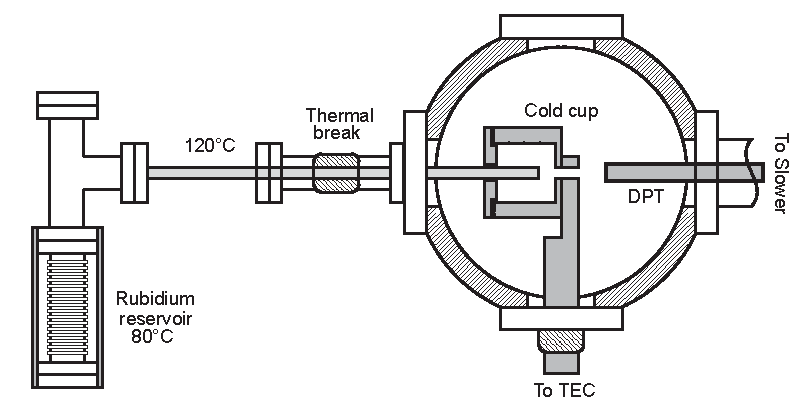
\includegraphics[width=0.48\textwidth]{figs/oven.pdf}
\caption{{\color{red} taken from Andy's thesis.} This figure shows the rubidium atom source.}
\label{fig:oven}
\end{wrapfigure}

Rubidium atoms in a reservoir are heated in an oven to approximately $80\,^{\circ}\mathrm{C}$. The resulting vapour effuses through a heated drift tube and is then incident on a `cold-cup'' aperture resulting in a collimated beam. At this point the atoms have a velocity in the region of 300m/s. This is shown in figure \ref{fig:oven}


\subsection{Zeeman Slower}
The Zeeman slower cools the atoms atoms from having a velocity of order 300m/s to 35m/s. This is achieved with doppler cooling using red-detuned light. As the atoms slow down the resonance condition changes so a magnetic coil with a tapered pitch is used to maintain the interaction. Another solution which is not implemented in this system is to use a frequency `chirp' in the cooling light.

An Eagleyards tapered amplifier seeded with light from two \glspl{ecdl} is used for the doppler cooling. The first \gls{ecdl} produces the cooling light and the second is used to repump any atoms that fall into a dark state.

The \gls{ecdl} is locked to the appropriate frequency using a saturated absorption configuration\cite{maguire_theoretical_2006,haroche_theory_1972, preston_doppler-free_1996}.

\subsection{Quasi-Mirror Magneto-Optic Trap}
\glspl{mot} have been used extensively in atom-optics laboratories to trap and cool atoms of many species. The physics of \glspl{mot} is well documented and understood\cite{metcalf_laser_1999}.

A conventional \gls{mot} consists of six beams which are able to damp the velocity of atoms is all directions where the beam overlap. A simpler design using only four beams is the ``mirror-MOT''. Mirror-MOTs typically suffer from a reduced trapping volume\cite{reichel_atomic_1999}.

In the \gls{caes} the accelerating structure required to extract the electron bunches is integrated with the mirror-MOT, ``Quasi-Mirror Magneto-Optical Trap'' (QMMOT)\cite{hanssen_using_2006}. Figure \ref{fig:qmmot} shows a schematic of the QMMOT where one of the plates is transmissive and the other reflective and both can be charged to provide the accelerating electric field.

\begin{figure}[h]
\centering
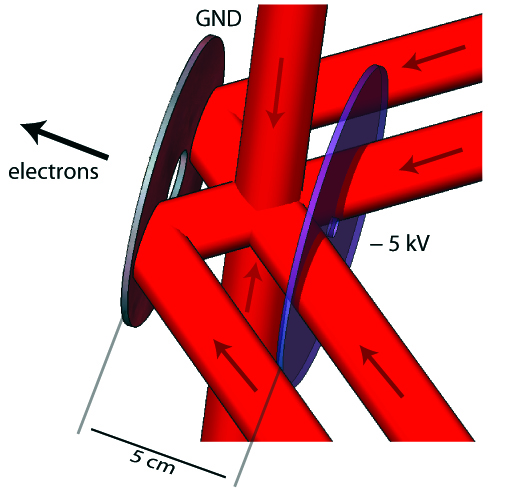
\includegraphics[width=0.45\textwidth]{figs/qMMOT.jpg}
\caption{{\color{red}Also taken from Andy's thesis.}Quasi-Mirror Magneto-Optical Trap. Two of the horizontal cooling beams are reflected from the conductive mirror and the other two pass through the conductive window to form the trapping region. To extract electrons a static electric field is applied once the cloud has been ionised.}
\label{fig:qmmot}
\end{figure}

The laser power for the \gls{mot} is supplied by a Toptica \gls{ta} seeded by the cooling and repump \glspl{ecdl} which are locked onto the appropriate atomic transistions using saturated absorption setups. A pair of magnetic coils external to the vacuum system in an anti-Helpholtz configuration proved the magnetic fields for the \gls{mot}.

\section{Electron Generation}

The generation of electrons is a central part of the \gls{caes} and each of the two stages has its own light source.

\subsection{Excitation}

The excitation of the atoms in the cloud can be done in one of two ways in the \gls{caes}. The first method of excitation is a $50\,\unit{\mu s}$ exposure of light from an \gls{ecdl} and the second method is to use a pulse from a Newport 3960 fs Tsunami which is able to produce $35\,\unit{fs}$ long bunches.

\subsubsection{Continuous Excitation}

The \gls{ecdl} is locked onto the $5 ^2 S_{3/2} F=3\rightarrow5 ^2 P_{3/2} F=4$ transition of rubidium using saturated absorption and the exposure is controlled with an \gls{aom}. The excitation \gls{ecdl} beam shares much of its beam path with that of the femtosecond laser and a mirror on a flip mount is used to determine which used for excitation at a given time.The exposure of the atoms to the excitation beam is controlled with an \gls{aom} and is approximately $80\,\unit{\mu s}$ long.

\subsubsection{Femtosecond Excitation}

The Newport 3960 fs Tsunami produces approximately $80\,\unit{fs}$ long pulses of light with a wavelength centered around $800\,\unit{nm}$ with a $20\,\unit{nm}$ linewidth.\cite{mcculloch_towards_2012} Femtosecond excitation allows the \gls{caes} to produce electron bunchs that are picoseconds long.

\subsection{Shaping}

The \gls{caes} has the ability to create shaped electron bunches. This is done by applying a phase mask to the excitation beam with a \gls{slm}. The shaped excitation beam causes the distribution of excited atoms in the atom cloud to be proportionally shaped. This results in electron bunches with the same shap as the excitation beam.

\begin{figure}[h]
\centering
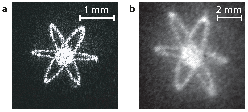
\includegraphics[width=0.5\textwidth]{figs/atom_electrons.pdf}
\caption{{\color{red}from Andy's thesis.}Shaped electron bunches produced by the Melbourne CAES. Image a) shows the exitation laser intensity profile. b) shows the measured electron density distribution.}
\end{figure}

\subsection{Ionisation}



\section{Sample Chamber}
text
    \subsection{Beam Steering and Focussing}
text

    \subsection{Detector}
text

\section{Electron Beam Steering}
At the start of this project the steering of the electron beam through the new sample chamber and onto the detector was being achieved with a large iron permanent magnetic. As a side project a quadrupole magnetic steering device was designed and constructed to allow more precise and repeatable control over the electron beam.

In order to get an idea of the strength of magnetic field required for this device the magnetic terrain outside the electron path was measured with a Hall probe. The field was found to vary considerably around the steel vacuum system, mechanincal and electrical mechanical devices. It was possible however to determine the approximate strength of field that the steering device would have to deal with. The magnetic field around the electron path has an average of $0.68\,\unit{G}$ and a standard deviation of $0.57\,\unit{G}$.

In order to control the electron trajectories steering on both axes is required. and the simplest way to achieve this is with two pairs of current carrying wires as shown in figure \ref{fig:mag_steering}. Realistically instead of using single wires bundles of wires will be used. The magnetic field at the midpoint between a pair of wire bundles, each with $n$ wires, is
\begin{equation}
B=\frac{2n\mu_0I}{\pi d}
\end{equation}
where $\mu_0$ is the permeability of free space, $I$ is the current in the wire and $d$ is the distance between the two wires.

The is possible to put the bundles of wires $70\,\unit{mm}$ from the centre of the vacuum system. Using a reasonable current of $0.5\,\unit{A}$ and generating a field equal to the average magnetic field of $0.68\,\unit{G}$ would require $23.8$ wires in each of the wire bundles.

\begin{figure}[h]
\centering
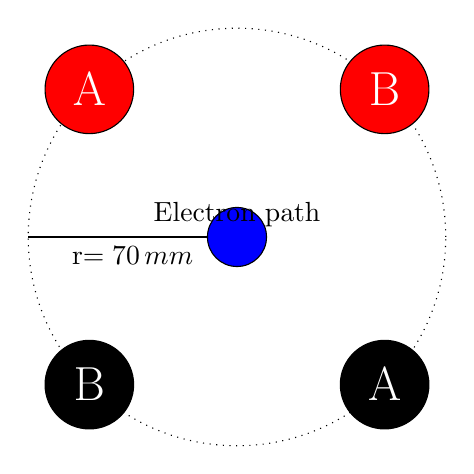
\begin{tikzpicture}
    \begin{scope}[scale=0.75]
        \draw[dotted] (0,0) circle (3.535);
        \draw (0,0) -- node[below] {r$=70\,\unit{mm}$} (-3.535, 0);

        \filldraw[fill=blue] (0,0) circle (0.5) node[above=0.3] {Electron path};

        \filldraw[fill=red] (2.5, 2.5) node[white] {\LARGE B} circle (0.75);
        \filldraw[fill=black] (-2.5, -2.5) node[white] {\LARGE B} circle (0.75);
        \filldraw[fill=red] (-2.5, 2.5) node[white] {\LARGE A} circle (0.75);
        \filldraw[fill=black] (2.5, -2.5) node[white] {\LARGE A} circle (0.75);
    \end{scope}
\end{tikzpicture}
\caption{Two pairs of current carrying wires (A and B) used to steer the electrons which are directed into the page. The current in the red wires is in the opposite direction to that in the black wires.}
\label{fig:mag_steering}
\end{figure}

Two pairs of steering coils, each with 25 turns, were constructed to implement this design. Each pair of wire bundles in joined together and to the power supply well away from the vacuum system to avoid disturbing the magnetic steering. The coils are mounted onto the vacuum system using plastic collars that were created by the department's workshop and the wires were confined in $20\,\unit{mm}$ electrical conduit.

Typical currents that are sufficient to steer the electrons onto the detector are for one axis $1.76\,\unit{A}$ and $1.52\,\unit{A}$ for the other. These values are much higher that the estimated but well within the capabilities of the device.

\section{Optical Dipole Trap}

The design of the \gls{odt} began in 2011 and the first trapping was observed in late 2012.
{\color{red} more stuff}

\subsection{Tapered Amplifier}
The \gls{ta} serves as the light source for the \gls{odt} and is built from an Eagleyard Photonics $780\,\unit{nm}$ $2\,\unit{W}$ CR-Mounted \gls{ta} seeded by a homebuilt \gls{ecdl}. This method of seeding \glspl{ta} is known as a \gls{mopa}\cite{wilson_narrow-linewidth_1998}. Due to a change in the mounting of the \gls{ta} chip it was necessary to redesign part of David Sheludko's \gls{mopa} design\cite{sheludko_shaped_2010}. A number of other changes to the original \gls{mopa} design were also made to allow more flexibility during alignment. It was also necessary to build a new \gls{mopa} from the new and existing parts.

{\color{red} more details? pictures?}

The \gls{ecdl} provides approximately $25\,\unit{mW}$ of injection seed with a linewidth typically below $300\,\unit{kHz}$. The seed laser is focussed onto the input facet of the \gls{ta} with a high \gls{na} lens\footnote{Thorlabs C230TM-B f=$4.5\,\unit{mm}$ $0.55\,\unit{NA}$}. The beam from the output facet of the \gls{ta} is collimated with two lens due to the high astigmatism in the output beam. The first lens is a high \gls{na} aspheric lens\footnote{Thorlabs C330TM-B f=$3.1\,\unit{mm}$ $0.68\,\unit{NA}$} and the second is a cylindrical lens\footnote{Unknown provenance f=$50\,\unit{mm}$} to counter the horizontal divergence. The outgoing beam then passes through a double stage optical isolator to prevent optical feedback causing damage to the \gls{ta}. The maximum output power of the \gls{ta}, after the isolator, is approximately $1.75\,\unit{W}$.

A small portion of the seed beam is siphoned into a saturated absorption setup\cite{maguire_theoretical_2006, haroche_theory_1972, preston_doppler-free_1996} to allow locking of the seed beam to the resonances of rubidium. This is not particularly useful during normal operation since the laser is usually detuned well beyond the resonances however it is useful during alignment as discussed below. When the \gls{ta} is running optical feedback interferes with the \gls{ecdl} causing further issues with visually deciphering, let alone locking to, the saturated absorption signal.

The output beam is coupled into a polarisation maintaining, single-mode fibre with the output end at the main experiment. At maximum power the power of the beam out of the fibre is approximately 40\% of the input power. Most of the power loss is due to the non-Gaussian profile of the \gls{ta} beam. While 60\% of the power is lost the major advantage of fibre coupling the beam is that the output beam is almost perfectly Gaussian in profile which is a necessity for \glspl{odt}.

A fraction of a percent of the light reflecting off the final mirror before the fibre mount transmits through the mirror. This light is incident on a wavemeter and is used to monitor the wavelength of the output beam as well as check that the light is of a single wavelength. Occasionally the seed laser will operate in two modes simultaneously and the \gls{ta} amplifies both modes which makes the trapping less predictable.

An old hard disc drive was used to create a shutter\cite{scholten_enhanced_2007} that is connected to the computer that runs the experiment. The shutter has a response time of $6\,\unit{ms}$ which must be taken into account when scheduling the timing of the experiment.

The \gls{ta}'s performance is sensitive to temperature so it is maintained at a constant temperature with water cooling and a \gls{tec} controlled by a Thorlabs temperature controller\footnote{Thorlabs TED200 C}. The \gls{ecdl} is controlled and powered by a Moglabs Diode Laser Controller and the \gls{ta} is powered by a ThorLabs laser diode controller\footnote{Thorlabs LDC 240 C}.

\begin{figure}[h]
\centering
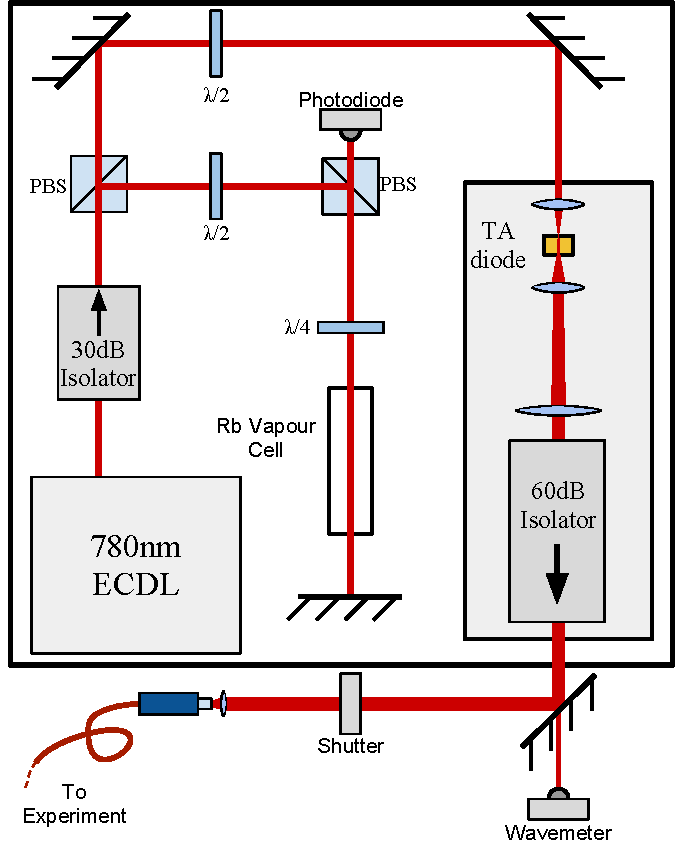
\includegraphics[width=0.5\textwidth]{figs/TAsetup.pdf}
\caption{The configuration of the light source for the close to resonance optical dipole trap. The tapered amplifier (TA) is seeded by the external cavity diode laser (ECDL). A portion of the seed beam is directed into a saturated absorption setup which, due to the detuning of the ECDL, is usually not useful. A tiny portion of the amplified beam transmits through the final mirror and is incident on the input to a wavemeter. A computer controlled shutter is used to turn the trapping beam on and off. The amplified beam has been coupled into a polarisation maintaining, single mode fibre.}
\end{figure}

\subsection{Fiber laser}

A Keopsys $20\,\unit{W}$ \gls{cw} fibre laser could also be used as a light source for \gls{odt}. Using this light source would significantly reduce the scattering rate and thus provide longer trap lifetimes. The potential depth of the trap would be reduced and this would result in a smaller effective trapping volume.

Another issue with the $20\,\unit{W}$ fibre laser is safety. $780\,\unit{nm}$ light is visible unlike $1064\,\unit{nm}$ light which is well into the infrared spectrum. This combined with the huge power of this \gls{cw} laser would mean that great care must be taken with the design and operation of beam lines. The laser would also be capable of damaging some optical components.


\subsection{Optical Dipole Trap}

\Gls{odt} consist of focussed Gaussian laser beams. The output of the \gls{ta} fibre provides a Gaussian beam and the focussing optics described in this section produce the focussed beam.

The output end of the \gls{ta} fibre is mounted in a cage to allow precise alignment of lens for focussing (the `objective' lens) and beam expansion and shrinking. While the potential for shrinking and expanding the beam incident on the objective lens is available it was not used in the final configuration.

There is a limited amount of optical access to the \gls{mot} available and the \gls{odt} used two almost orthogonal beam paths the second of which is shared with the $480\,\unit{nm}$ ionisation laser. Both of the paths are approximately $60^{\circ}$ from horizontal. All the windows to the vacuum system are \gls{ar} coated for $780\,\unit{nm}$ light.

The distance from one window to the opposite is $412.3\,\unit{mm}$ and the \gls{mot} should be situated halfway between them. The objective lens\footnote{Thorlabs AC508-250-B-ML f=$250\,\unit{mm}$} have a focal length of $250\,\unit{mm}$ which gives sufficient space to allow for adjustments of the beam waists. After the window of the first beam is another $250\,\unit{mm}$ lens to re-collimate the beam. This collimated beam is then propagated through free space to the second beam axis.

The second beam axis is shared with the blue, nanosecond-pulse ionisation laser. A long-pass dichroic mirror\footnote{Thorlabs DMLP567L} is used to combine the two beam paths. The focussing optics for the ionisation and the \gls{odt} path are located before the dichroic. The objective lens for the second beam of the \gls{odt} is a $300\,\unit{mm}$ lens due to the extra distance imposed by the dichroic.

As mentioned in \ref{odt_polarisation} the polarisation of the second beam must be orthogonal to that of the first to avoid standing waves and this is achieved with a half-waveplate as indicated in figure \ref{fig:dipole_rig}.

After the second trapping beam has left the vacuum system it is incident on a power meter. The power meter operates with a reflective attenuator and the reflected beam is incident on a photodiode that is used for timing measurements. The final reflection off of the photodiode is safely disposed of with a beam stop.

\begin{figure}[h]
\centering
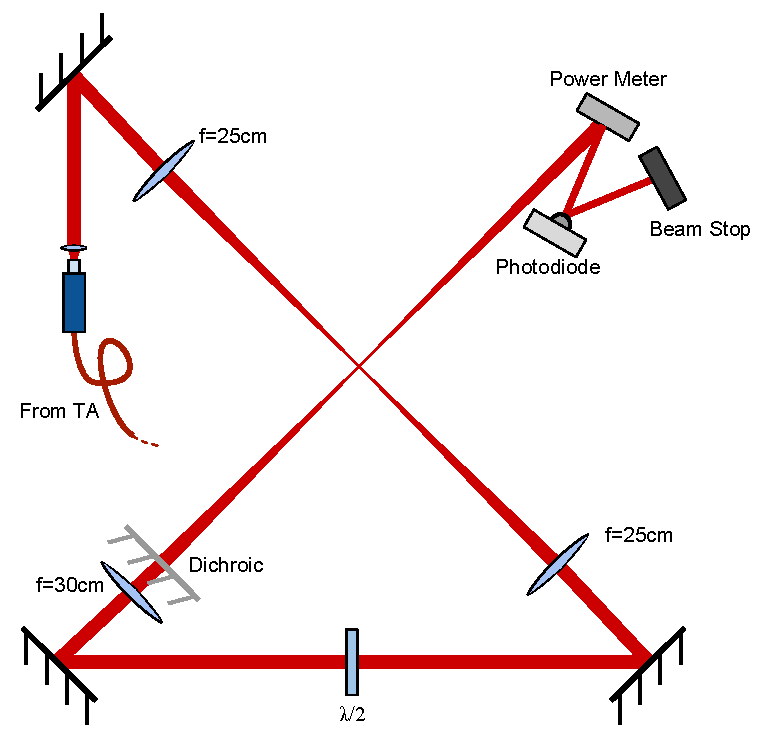
\includegraphics[width=0.4\textwidth]{figs/DipoleTrapRig.pdf}
\caption{The ODT beam path originates with the output of the TA fibre. The beam is then focussed by an objective lens and passed through the vacuum system with the beam waist at the MOT. As the beam leaves the vacuum system it is recollimated and recycled for the second beam of the ODT. The polarisation is rotated with a half-waveplate and the beam is again focussed at the MOT. The beam also passes through a dichroic mirror so that the optical access can be shared with the blue ionisation beam. A power meter and photodiode are located at the end of the beam path to allow for diagnostics and the beam is terminated with a beam stop.}
\label{fig:dipole_rig}
\end{figure}

\subsubsection{Alignment}

The alignment of the crossed \gls{odt} is done but first tuning the seed \gls{ecdl} close to resonance such that when the laser is scanning the saturated absorption signal is visible on the \gls{cro}. With the detuning this low the scattering rate becomes very large and portions of the \gls{mot} are visibly blown away by the \gls{odt} beams when viewed by the \gls{ccd} cameras that monitor fluorescence. An example of this is shown in figure \ref{fig:mot_slice}. The level of effect the \gls{odt} beams have on the trapped atoms can be varied by altering the current in the \gls{ta} and the detuning of the \gls{ecdl}. This process allows the two beams to be overlapped in the region of the \gls{mot}.

\begin{figure}[H]
\centering
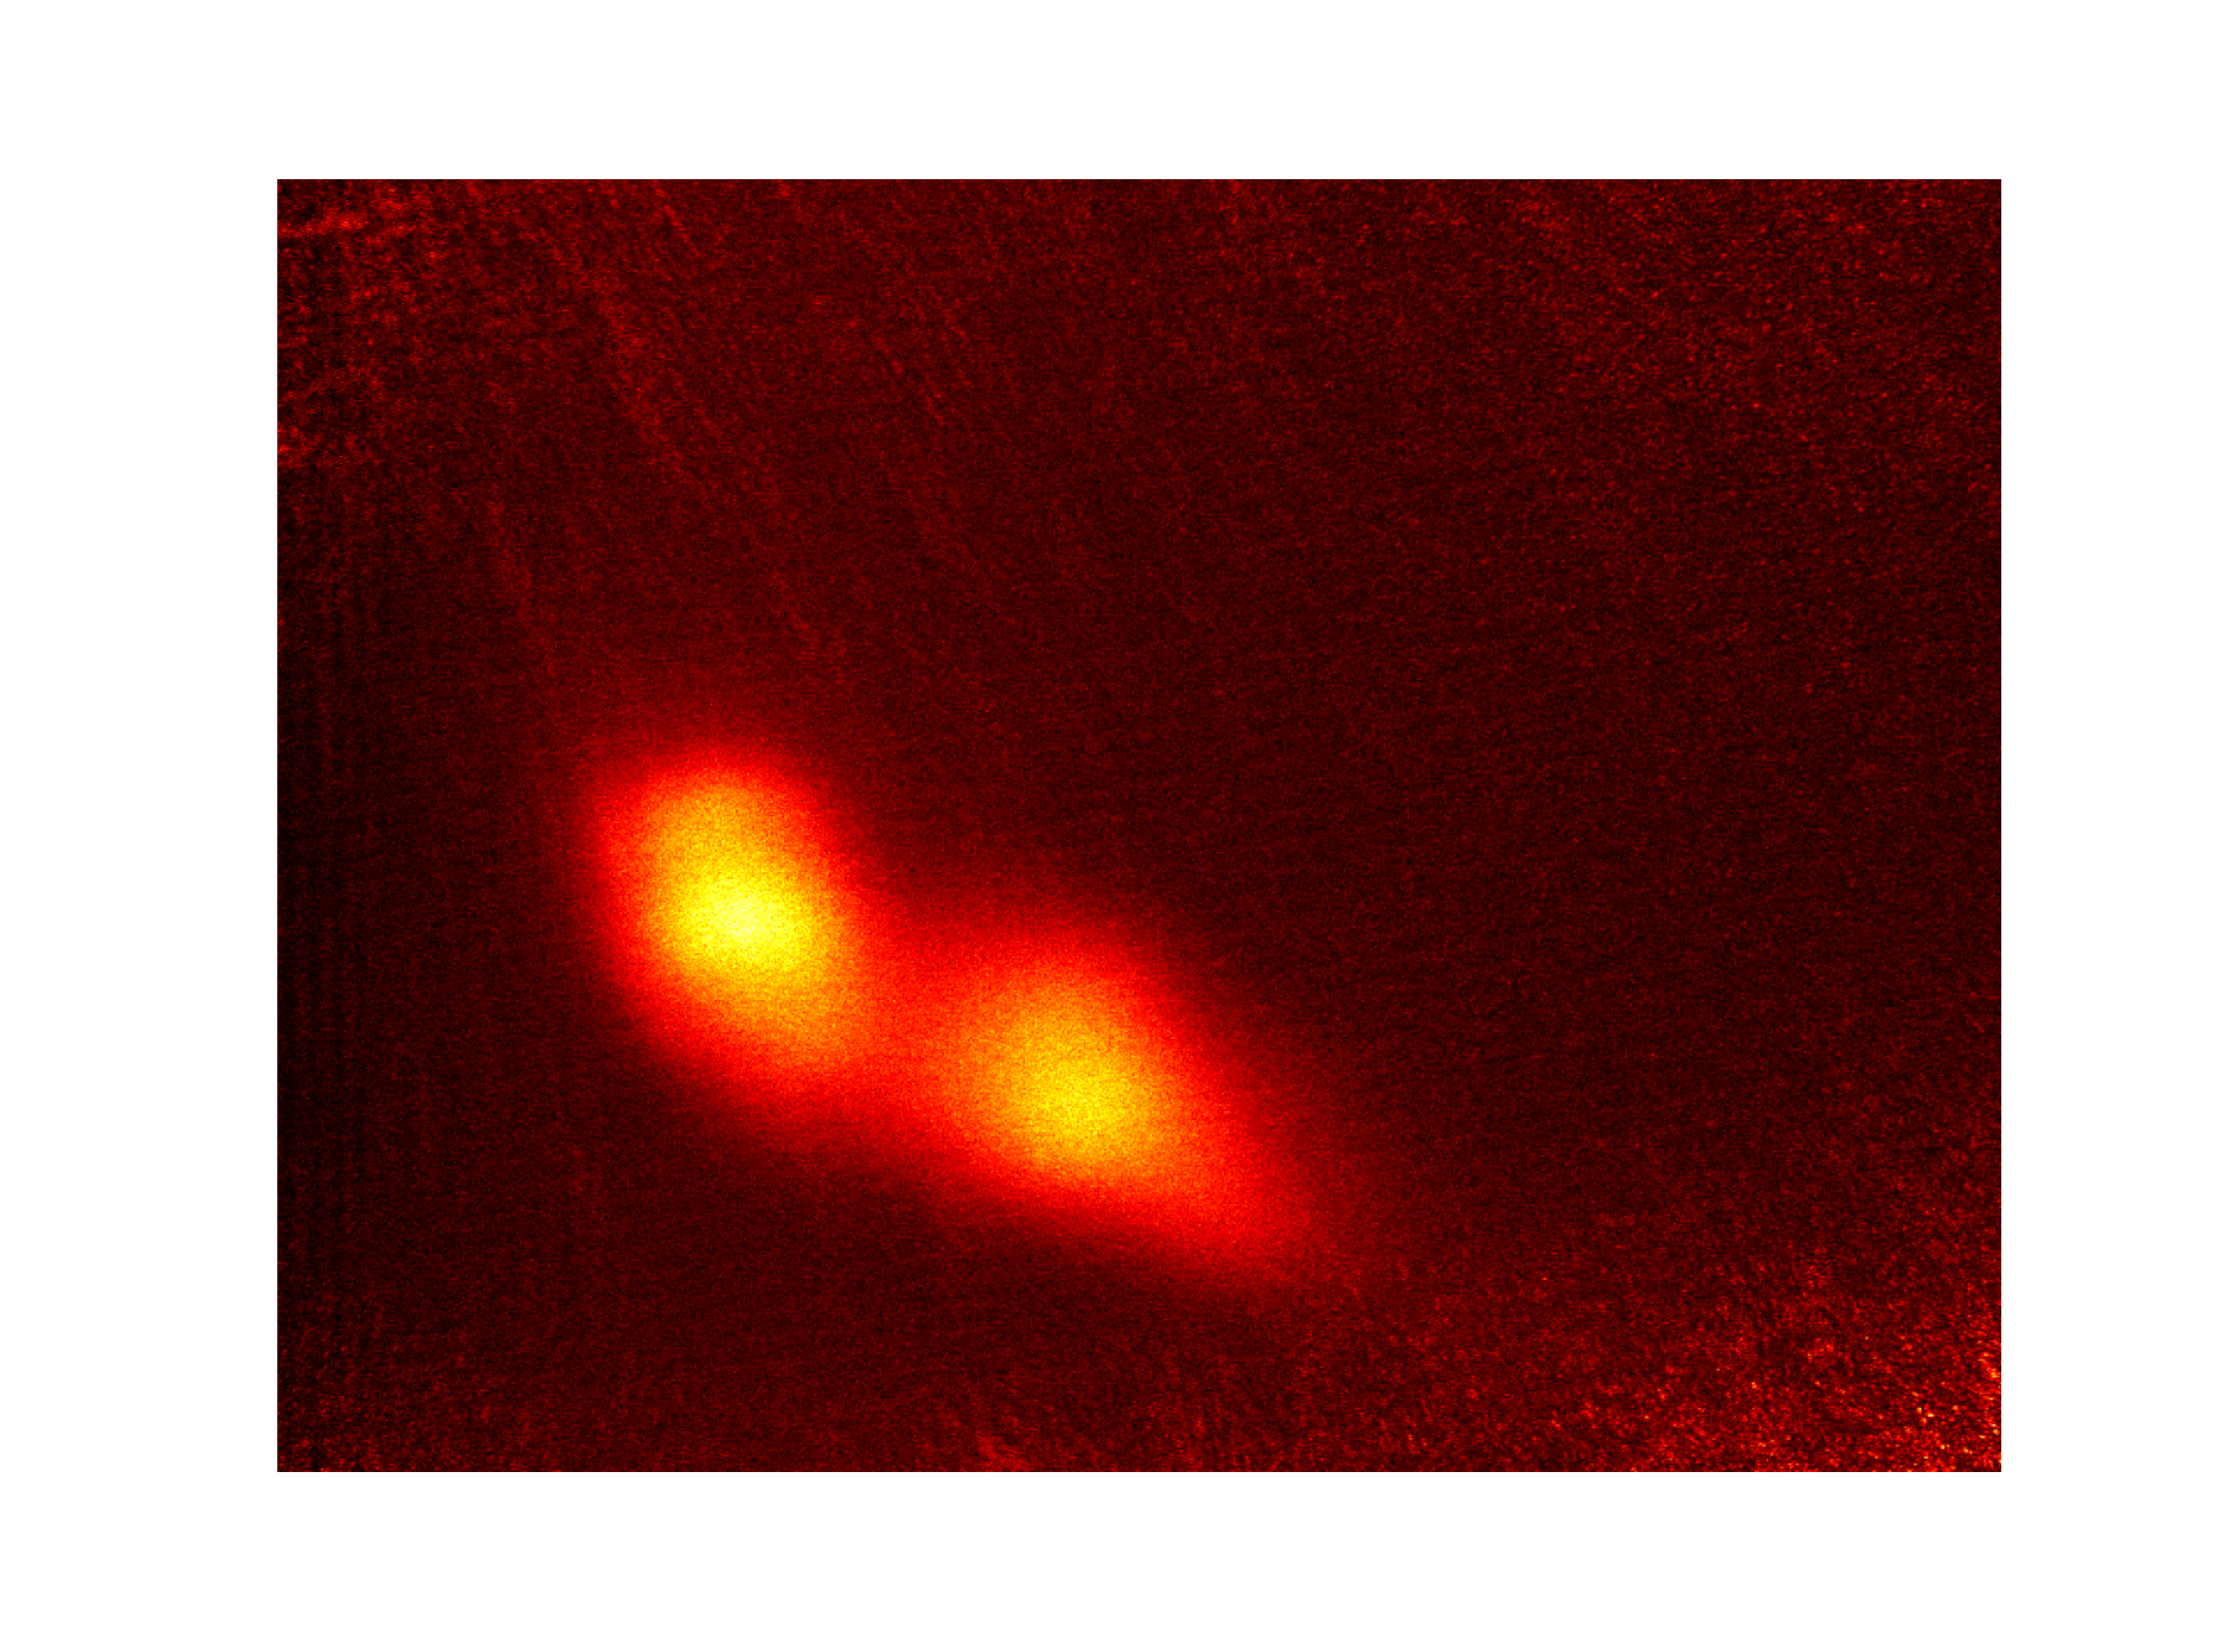
\includegraphics[width=0.3\textwidth]{figs/mot_slice.pdf}
\caption{The first beam of the ODT dividing the MOT into two halves.}
\label{fig:mot_slice}
\end{figure}

\section{Absorption Imaging}

In order to detect trapping within the \gls{odt} it is necessary to have a way of imaging it. Fluorescence imaging is not sufficient due to the fact that the detuned beams of the \gls{odt} do not induce visible amounts of fluorescence. Absorption imaging however is able to image the \gls{odt}.

The light source for imaging is shared with the continuous excitation beam and is an \gls{ecdl} locked with saturated absorption and controlled by a Mogbox\footnote{Moglabs Diode Laser Controller}. The power available for imaging can vary from a few microWatts to $2.5\,\unit{mW}$ depending on the position of the half wave plate located before the \gls{pbs} that splits the beam between the imaging and excitation beam lines. The imaging beam is then coupled into a fibre and brought over to the main experiment.

The imaging beam shares optical access with the vertical \gls{mot} beam. By putting the imaging beam slightly off axis compared to the \gls{mot} beam it is possible to insert and extract the beam without impact on the trapping beam.

A camera lens\footnote{Nikon AF Micro-Nikkor $200\,\unit{mm}$} is used to focus the beam onto a \gls{ccd} camera\footnote{Allied Vision Technologies Stingray F-080B}. The effective size of the camera's pixels was calibrated by first getting the camera to focus on a fluorescing \gls{mot}. Then a mirror was placed in the beam line near the camera and a normal ruler was placed so that it was visible on the camera and in-focus. In this situation the ruler is in a position equivalent to the \gls{mot} so by measuring the size of a pixel with the ruler we can later measure the size of features in the \gls{mot} plane. In this imaging beamline the effective pixel size was calculated to be $12.8\pm0.4\,\unit{\mu m}$.

\begin{figure}[H]
\centering
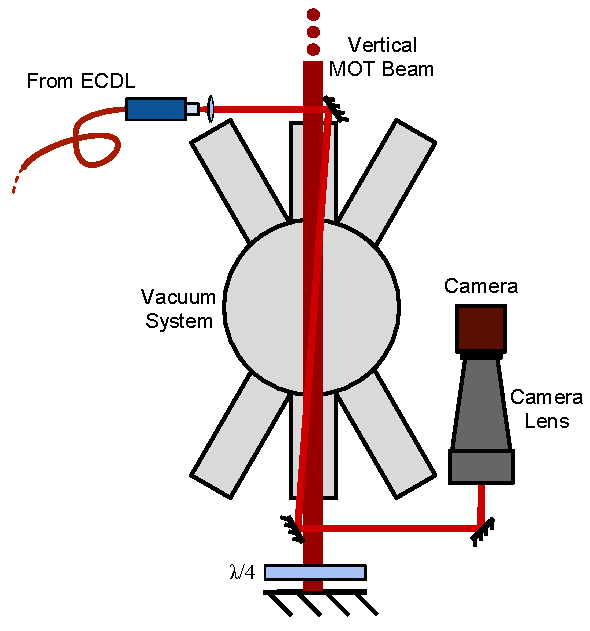
\includegraphics[width=0.5\textwidth]{figs/ImagingRig.pdf}
\caption{The imaging beam's optical access is shared with the vertical MOT beam. The beam is collimated from a fibre and is slightly off axis from the MOT beam. It is recorded by a Stingray CCD camera after being focussed by a Nikon camera lens.}
\label{fig:imaging_rig}
\end{figure}

The axis the imaging beam images is not ideal. Ideally the imaging beam axis would be orthogonal to both of the trapping beam which allows clear images to be made of both beams. Having the imaging axis orthogonal to gravity also allows the observation of atom clouds falling. Unfortunately it is not currently feasable to put the imaging beam on the horizontal axis, which would meet these criterion. This is due to the scarcity of optical access on that axis and the crowded nature inside the vacuum system. As the results in chapter 4 show it is still possible to differentiate between the two beams due to the off-axis alignment of the imaging beam.

{\color{red} mention backgrounds}

\section{Software}

In order to perform absorption imaging new software was required to communicate with the AVT camera and to do the image analysis. This new software was created in Labview and Python.

The software for image acquisition, integration and absorption imaging was created in Labview and is able to acquire images from the camera and apply the theory described in section \ref{sec:absorption_imaging} in order to immediately present the user with the absorption images (such as the one in figure \ref{fig:absorption_example}). The Labview software is also able to present the atom count for a given absorption image.

More in-depth analysis, such as temperature measurements, is performed using Python programs described in more detail in chapter 4.

\section{Experimental Procedure}

During standard operation the \gls{caes} operates at a frequency of $10\,\unit{Hz}$. This cycle consists of:
\begin{enumerate}
\item Loading  the \gls{mot} for approximately $93\,\unit{ms}$.
\item Turning off the magnetic and optical trapping.
\item Turning on the excitation laser (\gls{cw}).
\item $10\,\unit{ns}$ Ionisation pulse.
\item Turning the accelerating electric field on for $60\,\unit{\mu s}$.
\item Turning off the excitation laser and turning the magnet and optical trapping back on.
\end{enumerate}

When aligning, imaging and configuring the \gls{odt} the process changes. The ionisation and acceleration steps are not necessary and more steps are required for imaging. The state of each of the lasers and coils during this process is shown in figure \ref{fig:sequence}.

The longest step is the loading of the \gls{mot} which require both the Zeeman and \gls{mot} cooling. The \gls{odt} beam is also on during this stage so that the \gls{odt} can load. This step lasts for approximately $300\,\unit{ms}$ so that the \gls{mot} has plenty of time to load. 

In the next step atoms are held solely by the \gls{odt}. This step is of variable length depending on what is being examined. By imaging after a certain delay snapshops of the \gls{odt}'s evolution can be made.

In the imaging step the imaging laser is turned on and camera is triggered. It is important to turn the \gls{mot} repump laser on so that atoms do not fall into the dark state. The \gls{odt} laser is strong enough and the detuning small enough that it can act as a repump and excitation laser itself. To avoid potential confusion and to ensure that more atoms are able to be imaged it is best to turn off the trapping beam during imaging.

\begin{figure}[H]
\centering
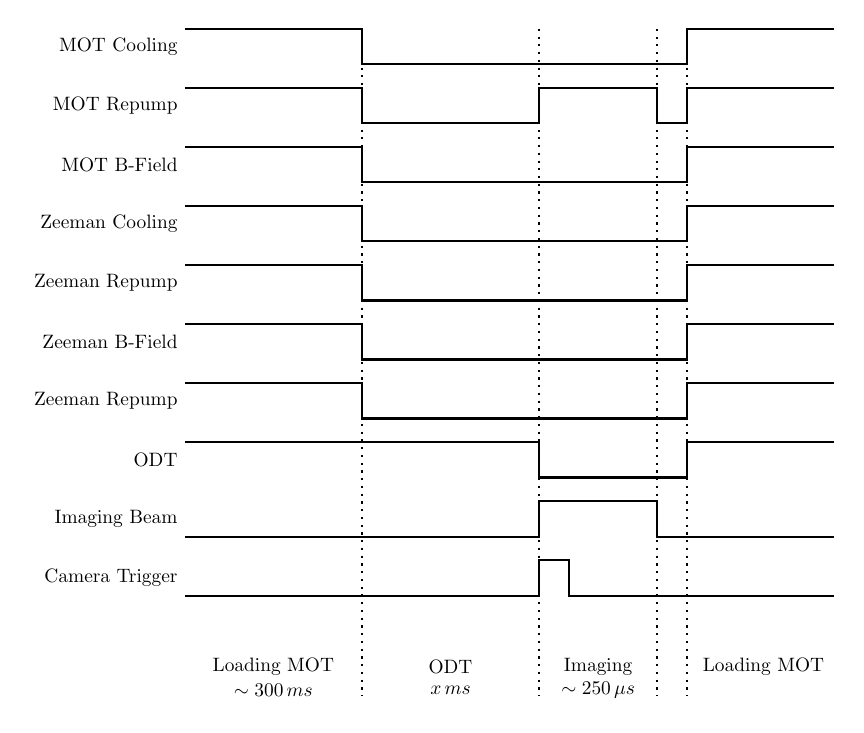
\begin{tikzpicture}[scale=0.75, every node/.style={scale=0.7}]
    \begin{scope}[thick, decoration={snake,amplitude=.4mm,
        segment length=2mm,post length=1mm}]
      \draw (0,10) node[left] {MOT Cooling};
        \draw (0,10.3)  -- (3, 10.3) -- (3, 9.7) -- (8.5, 9.7) -- (8.5, 10.3) -- (11, 10.3);

      \draw (0, 9) node[left] {MOT Repump};
        \draw (0, 9.3) -- (3, 9.3) -- (3, 8.7) -- (6, 8.7) -- (6, 9.3) -- (8, 9.3) -- (8, 8.7) -- (8.5, 8.7) -- (8.5, 9.3) -- (11, 9.3);

      \draw (0, 8) node[left] {MOT B-Field};
        \draw (0, 8.3) -- (3, 8.3) -- (3, 7.7)-- (8.5, 7.7) -- (8.5, 8.3) -- (11, 8.3);

      \draw (0, 7) node[left] {Zeeman Cooling};
        \draw (0, 7.3) -- (3, 7.3) -- (3, 6.7) -- (8.5, 6.7) -- (8.5, 7.3) -- (11, 7.3);

      \draw (0, 6) node[left] {Zeeman Repump};
        \draw (0, 6.3) -- (3, 6.3) -- (3, 5.7) -- (8.5, 5.7) -- (8.5, 6.3) -- (11, 6.3);

      \draw (0, 5) node[left] {Zeeman B-Field};
        \draw (0, 5.3) -- (3, 5.3) -- (3, 4.7) -- (8.5, 4.7) -- (8.5, 5.3) -- (11, 5.3);

      \draw (0, 4) node[left] {Zeeman Repump};
        \draw (0, 4.3) -- (3, 4.3) -- (3, 3.7) -- (8.5, 3.7) -- (8.5, 4.3) -- (11, 4.3);

      \draw (0, 3) node[left] {ODT};
        \draw (0, 3.3) -- (6, 3.3) -- (6, 2.7) -- (8.5, 2.7) -- (8.5, 3.3) -- (11, 3.3);

      \draw (0, 2) node[left] {Imaging Beam};
        \draw (0, 1.7) -- (6, 1.7) -- (6, 2.3) -- (8, 2.3) -- (8, 1.7) -- (11, 1.7);

      \draw (0, 1) node[left] {Camera Trigger};
        \draw (0, 0.7) -- (6, 0.7) -- (6, 1.3) -- (6.5, 1.3) -- (6.5, 0.7) -- (11, 0.7);

    \draw[dotted] (3, 10.3) -- (3, -1);
    \draw (1.5, -0.5) node {Loading MOT};
    \draw (1.5, -0.9) node {$\sim300\,\unit{ms}$};

    \draw[dotted] (6, 10.3) -- (6, -1);
    \draw (4.5, -0.5) node {ODT};
    \draw (4.5, -0.9) node {$x\,\unit{ms}$};

    \draw[dotted] (8, 10.3) -- (8, -1);
    \draw (7, -0.5) node {Imaging};
    \draw (7, -0.9) node {$\sim250\,\unit{\mu s}$};


    \draw[dotted] (8.5, 10.3) -- (8.5, -1);
    \draw (9.8, -0.5) node {Loading MOT};
    \end{scope}
\end{tikzpicture}
\caption{The experimental sequence used to examine the ODT.}
\label{fig:sequence}
\end{figure}

Another important consideration is the delay between a change in a control signal and response from a device (such as a laser, magnetic coil or camera). Lasers that are controlled with \glspl{aom} have a very fast repsonse time {\color{red} how fast? citation?}. The response time of the AVT camera has not been measured however it is significantly less than the usual exposure times of the camera (typically $30-100\,\unit{\mu s}$). The response times of the mechanical shutters used on the Zeeman slower and \gls{odt} however are significant.

The response times of the shutters can easily be measured by using a photodiode to compare the amount of light transmitting through the shutters with the signal controlling the shutter. {\color{red} should I meantion that this isn't my work? it was done by Paul and Rory} This method has shown that the response time of the Zeeman slower's shutter is $4.6\,\unit{ms}$ and the \gls{odt}'s shutter is $6.2\,\unit{ms}$. It is important to take these values into account when scheduling the timing of the experiment.

{\color{red} perhaps mention the apparent `blue trapping' we had when the trapping laser was acting as a repump}
